% !TEX root = Dokumentation.tex
\subsection{Risikomanagement}
Die Risiken, die während der Projektdurchführung entstehen könnten, sind im Folgenden aufgelistet. Um zu wissen, wie hoch ein Risiko eingeschätzt werden muss, wurde eine Grafik erstellt. Zu jedem Risiko sind auch Massnhamen aufgelistet, welche im Eintrittsfall unternommen werden können.
%
\begin{figure}[H]%Position festigen
\centering
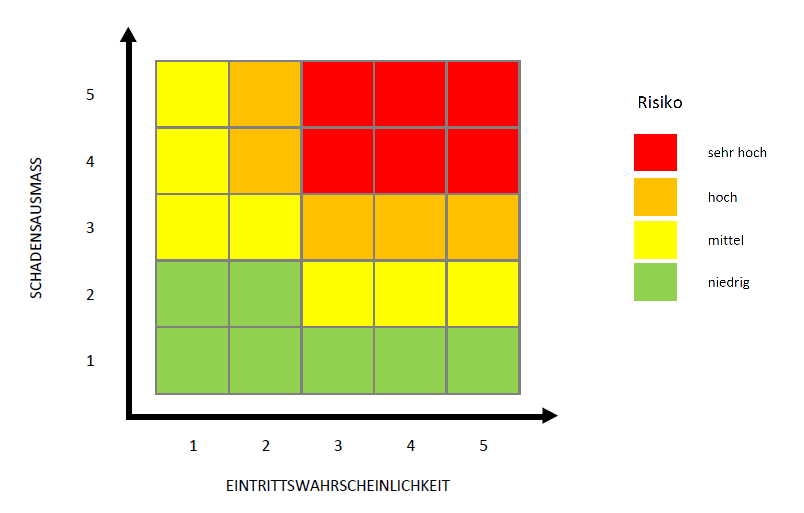
\includegraphics[width=0.8\textwidth]{Images/risikomatrix.png}
\caption{Risikomatrix}
\label{fig:Risikomatrix}
\end{figure}
%
\subsubsection{Risiken im Team}
\begin{table}[H]
\begin{tabular}{|p{0.3\textwidth}|p{0.2\textwidth}|p{0.2\textwidth}|p{0.2\textwidth}|}\hline	
% Titelzeile
	\textbf{Risiko}	& 	\textbf{Wahrscheinlichkeit} & \textbf{Schadensausmass}  & \textbf{Massnahmen} \\\hline
%
	Mitglied verlässt das Team	&	1	&	4	&	Neuverteilung der Arbeiten \\\hline
	Unzuverlässigkeit eines Teammitglieds	&	2	&	3-4	&	 Absprache im Team, um eine Lösung zu finden  \\\hline
	Unstimmigkeiten unter den Teammitgliedern	& 	3	&	4	& Absprache im Team, um eine Lösung zu finden, evtl. auch Rat von Supervisor einholen.  \\\hline
	Mitglied überlastet	&	4	&	3	&	Neuverteilung der Arbeiten \\\hline
	Kommunikationsprobleme	&	4	&	3	&	verbesserte Absprachen, Frequenz der Sitzungen erhöhen \\\hline
	Fehlende fachliche Kompetenz eines Mitglieds	&	2	&	2	&	Neuverteilung der Arbeiten \\\hline
	Fehlende soziale Kompetenz eines Mitglieds	&	1	&	3	&	Absprache im Team, um eine Lösung zu finden\\\hline
\end{tabular}
\caption{Risiken im Team}
\end{table}
%
\subsubsection{Risiken im Projektmanagement}
\begin{table}[H]
\begin{tabular}{|p{0.3\textwidth}|p{0.2\textwidth}|p{0.2\textwidth}|p{0.2\textwidth}|}\hline
%	
	\textbf{Risiko}	& 	\textbf{Wahrscheinlichkeit} & \textbf{Schadensausmass}  & \textbf{Massnahmen} \\\hline
		Missverständnisse bei den Anforderungen	&	3-4	&	3	& Absprache mit Supervisor  \\\hline
	Ineffizientes Arbeiten	&	3-4	&	2-3	& Neuorganisierung der Vorgehensweise  \\\hline
%	
	Überschreitung des Budgets	&	1	&	4	& Absprache mit Supervisor  \\\hline
\end{tabular}
\caption{Risiken im Projektmanagement}
\end{table}
%
\subsubsection{Risiken bei der Realisierung}
\begin{table}[H]
\begin{tabular}{|p{0.3\textwidth}|p{0.2\textwidth}|p{0.2\textwidth}|p{0.2\textwidth}|}\hline
%
	\textbf{Risiko}	& 	\textbf{Wahrscheinlichkeit} & \textbf{Schadensausmass}  & \textbf{Massnahmen} \\\hline
	
	Idee funktioniert nicht wie gewünscht	&	2	&	4	& neue Ideenfindung, Rat einholen  \\\hline
	Eingekaufte Komponente erfüllt Anforderung nicht	&	2	&	5	& andere Komponente einkaufen  \\\hline
		Projekt-anforderungen sind nicht erfüllt	&	1	&	5	&  Anpassungen planen \\\hline
		Bestellungen werden zu spät geliefert &	4	&	4	&  Versuchen andere Arbeiten vorzuziehen \\\hline
		Fertigungsaufträge werden zu spät geliefert &	4	&	4	&  Versuchen andere Arbeiten vorzuziehen \\\hline
		Defekte bei der Hardware &	2	&	4	&  Neu bestellen (Garantiebedingungen beachten) \\\hline
		Implementation dauert länger als geplant  &	3	&	3	&  Ausserhalb der Unterrichtszeit arbeiten \\\hline
		Festigkeisprobleme der produzierten Komponenten  & 2	&	5	&  neue Lösungen finden / anderes Material \\\hline
		Abnutzung der Zahnräder  & 2	&	4	&  neu drucken, neue Lösungen finden / anderes Material \\\hline
		Drehmoment des Motors reicht nicht aus & 2	&	4	&  neue Lösungen finden / anderer Motor verwenden \\\hline
		Fehler beim Print & 2	&	4	&  Print verbessern und neu in Auftrag geben \\\hline
		Ausfall von Komponten & 2	 &	4	&  neue Lösungen finden / andere Komponenten bestellen (je nach Zeitpunkt) \\\hline
		Greifer kann den Container nicht richtig greifen & 3	&	2	&  Greifer mit rutschfesten Material versehen \\\hline
		Verkabelungsprobleme & 3	&	3	&  neue Kabel, Neukonstruierung \\\hline
		Fahrbahnerkennung funktioniert zu ungenau & 2	&	3	&  Optimierung der Implementation \\\hline
		Falsche Objekte werden als Container identifiziert & 3&	2	&  Optimierung der Implementation, Bild zuschneiden \\\hline
		Distanz zu Container wird von der Bilderkennung zu ungenau berechnet & 2	&	3	&  Optimierung der Implementation \\\hline
		
\end{tabular}
\caption{Risiken bei der Realisierung}
\end{table}
%
\subsubsection{Andere Risiken}
\begin{table}[H]
\begin{tabular}{|p{0.3\textwidth}|p{0.2\textwidth}|p{0.2\textwidth}|p{0.2\textwidth}|}\hline
	%
	\textbf{Risiko}	& 	\textbf{Wahrscheinlichkeit} & \textbf{Schadensausmass}  & \textbf{Massnahmen} \\\hline
	%
	Lange Lieferzeiten bei Bestellungen	&	3	&	2	& andere Arbeiten aufnehmen, früher bestellen  \\\hline
	Github fällt aus	&	1	&	4	& Lokal weiterarbeiten  \\\hline
	Fahrzeug wird beschädigt	&	2	&	5	& je nach Ausmass neu fertigen  \\\hline
\end{tabular}
\caption{andere Risiken}
\end{table}